\documentclass[obeyspaces,spaces,hyphens,dvipsnames]{beamer}
\usepackage[utf8]{inputenc}
\usepackage{minted}
\usepackage{hyperref}

\mode<presentation>
\usetheme{FreeElectrons}

\newcommand{\codehack}[1]{{\usebeamercolor[fg]{code} {\tt #1}}}

\title{UBI/MLC: proposal to address the paired pages problem}
\authors{Boris Brezillon}
\institute{Free Electrons}

\setcounter{tocdepth}{2}

\begin{document}

\begin{frame}{UBI/MLC: addressing paired pages problem}
  \begin{center}
    \huge
    UBI/MLC: proposal to address the paired pages problem
  \end{center}
\end{frame}

\AtBeginSection
{
}

\AtBeginSubsection
{
}

\begin{frame}{UBI: detailing the problem}
  \begin{itemize}
  \item MLC chips are exposing 2 bits cells
  \item Each bit is assigned to a specific page in a block
  \item This is called page pairing
  \item Interrupting a write while writing on a page attached
        to the MSB will corrupt the page attached to the LSB
  \item Solutions to make write access reliable:
    \begin{itemize}
    \item Use hardware SLC mode
    \item Use software SLC mode
    \item Use MLC mode and copy the content of LSB pages
          somewhere else until MSB page has been programmed
    \end{itemize}
  \end{itemize}
\end{frame}

\begin{frame}{UBI: hardware SLC mode (current implementation)}
  \begin{itemize}
  \item Some MLC chips are providing an SLC mode feature
  \item Expose only 2 levels in each cells instead of 4
  \item Pros:
    \begin{itemize}
    \item Better read/write performances
    \item Better data retention (less impacted by read/write disturb)
    \item Easy to implement at the NAND level
    \end{itemize}
  \item Cons:
    \begin{itemize}
    \item MTD users have to know in advance how the erase block has been
	  be programmed (or try to read in MLC mode and fallback to SLC
	  mode if it doesn't work)
    \item Not supported on all NAND chips
    \end{itemize}
  \end{itemize}
\end{frame}

\begin{frame}{UBI: software SLC mode (part of new solution)}
  \begin{itemize}
  \item All pages attached to the MSB are manually skipped
  \item Pros:
    \begin{itemize}
    \item Works for all NANDs as long as we know the pairing scheme
    \item Erase block type can be detected at the UBI level without
          without having to test one mode before falling back to the
	  other
    \item Easy to implement at the NAND level
    \item Pairing scheme easily exportable at the MTD level
    \end{itemize}
  \item Cons:
    \begin{itemize}
    \item Less reliable and less performant than the hardware SLC
          mode approach
    \end{itemize}
  \end{itemize}
\end{frame}

\begin{frame}{UBI: copy LSB page (Micron's approach)}
  \begin{itemize}
  \item We are using all blocks in MLC mode
  \item All pages attached to the LSB are saved/copied to other block
        so that we can recover them in case of interrupt write on the
	MSB page
  \item Pros:
    \begin{itemize}
    \item Can work on all chips (but the implementation should be
          generic, which is not the case in Micron's proposal)
    \item ???
    \end{itemize}
  \item Cons:
    \begin{itemize}
    \item Lower performances even more than the software SLC mode
          approach (you have to write the data twice). Performances
	  can be improved with multi-plane read/program, but this adds
	  a dependency on this feature which is not supported on all
	  chips/controllers
    \item Flash storage utilization is not so good: for each partially
          written erase block you have to keep a backup erase block
    \item Hard to implement in a generic manner, and requires some
          invasive changes at the UBI/MTD and NAND layers
    \end{itemize}
  \end{itemize}
\end{frame}

\begin{frame}{UBI: SLC vs MLC mode}
  \begin{center}
    \includegraphics[scale=0.3]{ubi-slc-vs-mlc.pdf}
  \end{center}
\end{frame}

\begin{frame}{UBI: maximize storage usage with SLC mode}
  \begin{itemize}
  \item Mix MLC and SLC erase blocks
  \item Try to avoid data copy as much as possible
    \begin{itemize}
    \item Limits performance penalty
    \item Limits NAND wear
    \end{itemize}
  \item Solution: consolidate data in SLC erased block into MLC erase
        blocks when we start running out of free erase blocks
    \begin{itemize}
    \item No performance penalty and limits NAND wear when the NAND
          is relatively empty
    \item Provides a way to avoid corruption caused by interrupted
          PROGRAM on MSB pages
    \item Better flash storage usage compared to SLC only approach
    \end{itemize}
  \end{itemize}
\end{frame}

\begin{frame}{UBI: PEB consolidation}
  \begin{center}
    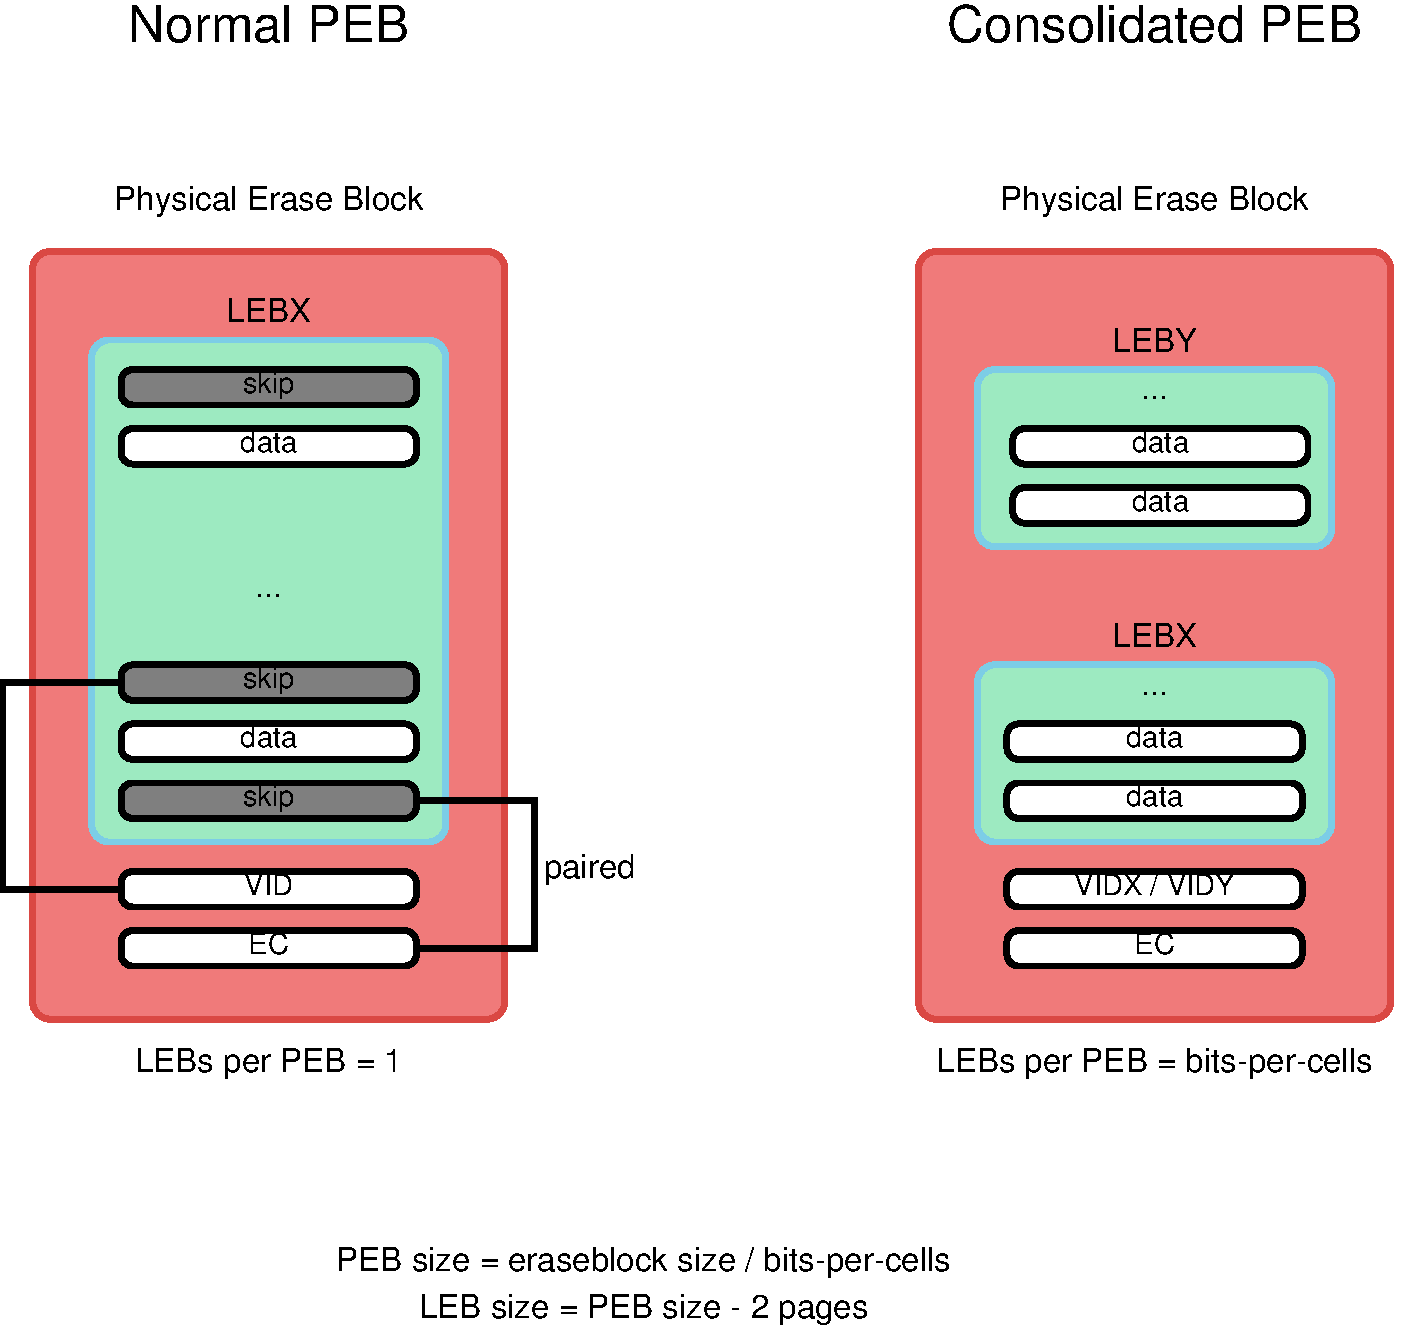
\includegraphics[scale=0.3]{ubi-peb-consolidation.pdf}
  \end{center}
\end{frame}

\begin{frame}{UBI: PEB consolidation workflow}
  \begin{center}
    \includegraphics[scale=0.3]{ubi-peb-consolidation-workflow.pdf}
  \end{center}
\end{frame}

\begin{frame}{UBI: PEB consolidation challenges}
  \begin{itemize}
  \item Try to limit the changes in UBI, and keep them well separated
  \item Add fastmap support
  \item Ensure that it works reliably on most (all?) MLC NANDs
  \item Find the correct consolidation threshold
    \begin{itemize}
    \item Too low: poor performances + NAND wear
    \item Too high: poor performances when the UBI partition reach it
          maximum capacity
    \end{itemize}
  \item Stress the implementation to ensure we're not missing some
        important case
  \item What happens when we only have partially written LEBs (those
        ones should not cannot be consolidated until they are full)?
  \end{itemize}
\end{frame}

\end{document}
